
\chapter{Adjustment of Light Amounts}

The light level from the master laser is constrained by our requirement that the Master laser operate single mode. However, we require control of the light levels further downstream in order to have the right light levels to avoid damage to the Acousto-Optic Modulator (AOM) and to have the right amount of light to injection lock the other lasers. 

A typical way to accomplish this is to install a half wave plate followed by a polarizing beam cube. In this way, one can take the linearly polarized incoming light and rotate its polarization to any angle. One can thus exert complete control of the amount of light coming out of the polarizing beam cube. 

We had initially intended to use this scheme. However, there was a mistake in placing the order. Instead of 0 order waveplates, we had received multi-order waveplates, whose performance rapidly degrades for wavelengths far from the specified wavelength. 

We could have easily ordered a 0 order waveplate to replace them. However, we found a way to use the exising wavelengths that was mildly interesting.

\subsection{A review of the principles of operation of a waveplate: }

Recall that a waveplate rotates polarization by changing the relative phase of the oscillating components of the incoming polarized light. A waveplate generally\footnote{and maybe always} has a fast axis and a slow axis. A half-wave plate is designed so that, at the specified wavelength, the component of polarization along the slow axis acquires a phase shift of $(2m+1)*\pi$ relative to the fast axis\footnote{here $m$ is an integer}. 

Recall that the phase acquired by light as it passes through a medium of index of refraction $n$ is given by 

\begin{equation}
  \Delta \phi = \frac{2 \pi n x}{\lambda} \label{deltaPhi0}
\end{equation}

Given indices of refraction of $n_1$ and $n_2$ for our two axes, we find that the difference in phase acquired by the components of the light's polarization will be 

\begin{equation}
\Delta \phi=\frac{2 \pi n_1 x}{\lambda} -\frac{2 \pi n_2 x}{\lambda}. \label{deltaPhi2}
\end{equation}

and we find that, in order to achieve the correct phase shift, the acceptable thicknesses of our half wave plate must satisfy

\begin{equation}
  \Delta \phi=(2m+1)\pi \label{deltaPhi1}
\end{equation}
where $m$ is the order of the waveplate.

Combining \ref{deltaPhi1} and \ref{deltaPhi2} we find that the thickness of a waveplate $x$ is given by

\begin{equation}
x=\frac{(2m+1) \lambda}{2 (n_1-n_2)}. \label{deltaPhi3}
\end{equation}


We now examine what will happen if we put a different wavelength than specified into the waveplate. Thus, we assume that $x$,$n_1$,$n_2$ and $m$ give the appropriate $\pi$ phase shift for the wavelength at which the waveplate is designed to work ($\lambda_s$). Now, we try light of a different wavelength, $\lambda'$. Assuming that the indices of refraction stay roughly the same for both $\lambda_s$ and $\lambda'$, we see that 

\begin{align}
\Delta \phi=\frac{2 \pi (n_1-n_2) x}{\lambda'} 
\end{align}
Then, taking $x\rightarrow ((2m+1) \lambda_s)/(2 (n_1-n_2))$ from Eq.\ \ref{deltaPhi3}, we get 
\begin{align}
\Delta \phi&=\frac{2 \pi (n_1-n_2) (2m+1) \lambda_s}{2 (n_1-n_2)\lambda'} \\
\Delta \phi&=\frac{\pi (2m+1) \lambda_s}{\lambda'} \label{deltaPhi4}
\end{align}
Eq.\ \ref{deltaPhi4} illustrates that the performance of a multi-order waveplate (with high value for $m$) will degrade more rapidly at different wavelengths than a low-order waveplate. 

In our lab, we had a half wave plate, but it was a multi-order plate designed for 405 nm. Thorlabs specifies that the waveplates we had\footnote{I know, put which ones exactly} will provide the correct retardance at 405 nm, however they also specify that at 407.71 nm the net retardance is 0.3655746 waves, or $\Delta \phi=(m_2+.3656) (2 \pi)$. Based on Eq.\ \ref{deltaPhi4}, we see that this is consistent with and $m=55$ order waveplate. 

The problem here is that, in order to completely control the amount of light getting to the AOM, we want to change the polarization from fully vertical to fully horizontal. Given that the incoming light is vertically polarized, this retardance does not allow us to get fully horizontally polarized light, thereby imposing a minimum amount of light on us, which was not welcome. 

However, we found that we can compensate for this by merely using two waveplates in series. Using numerical methods, we found that the user can fix the orientation of one of the waveplates in such a way that by rotating the other waveplate over some reasonable distance \footnote{i.e. over a range of angles large enough that rotating the waveplate by hand gives the user a decent amount of control}, the outgoing light can be made to smoothly transition between being completely vertical or completely horizontal\footnote{Though the states in between can be made to have any combination of horizontally polarized and vertically polarized light, the light that comes out in these states are not necessarily linearly polarized}

This can be demonstrated using the Jones matrix formalism. The polarization of the incoming light can be represented by the following Jones vector: 
\begin{equation}
\begin{pmatrix}
0\\1
\end{pmatrix}
\end{equation}

The Jones matrix corresponding to our waveplate is easily derived. Given the : 

\begin{multline}
\begin{pmatrix}
\cos\theta & - \sin \theta \\
\sin \theta & \cos\theta \\
\end{pmatrix}
\begin{pmatrix}
\xi & 0 \\
0 & 1 \\
\end{pmatrix}
\begin{pmatrix}
\cos\theta &  \sin \theta \\
-\sin \theta & \cos\theta \\
\end{pmatrix} \\
=
\begin{pmatrix}
\cos ^2 \theta+\xi \sin^2 \theta &  \cos\theta \sin \theta-\xi \cos\theta \sin \theta \\
\cos\theta \sin \theta-\xi \cos \theta \sin\theta & \xi \cos^2 \theta + \sin^2 \theta \\ \label{JonesMatrix001}
\end{pmatrix}
\end{multline}

where $\theta$ is the angle between the fast axis and the x axis. 

We let $\xi\approx e^{.366 (2 \pi)}$ as specified by the waveplate. Then, to represent two of them mounted at angles $\theta_1$ and $\theta_2$ respectively, we need merely multiply two matrices like the one in Eq.\ \ref{JonesMatrix001}. Writing out the result is simple, but probably not overly enlightening. 

By numerical experimentation, we found that there was a set of angles where we could mount our two waveplates that would result in a polarization for the outgoing light that is orthogonal to the polarization of the incoming light. 

\begin{figure}
    \centerline{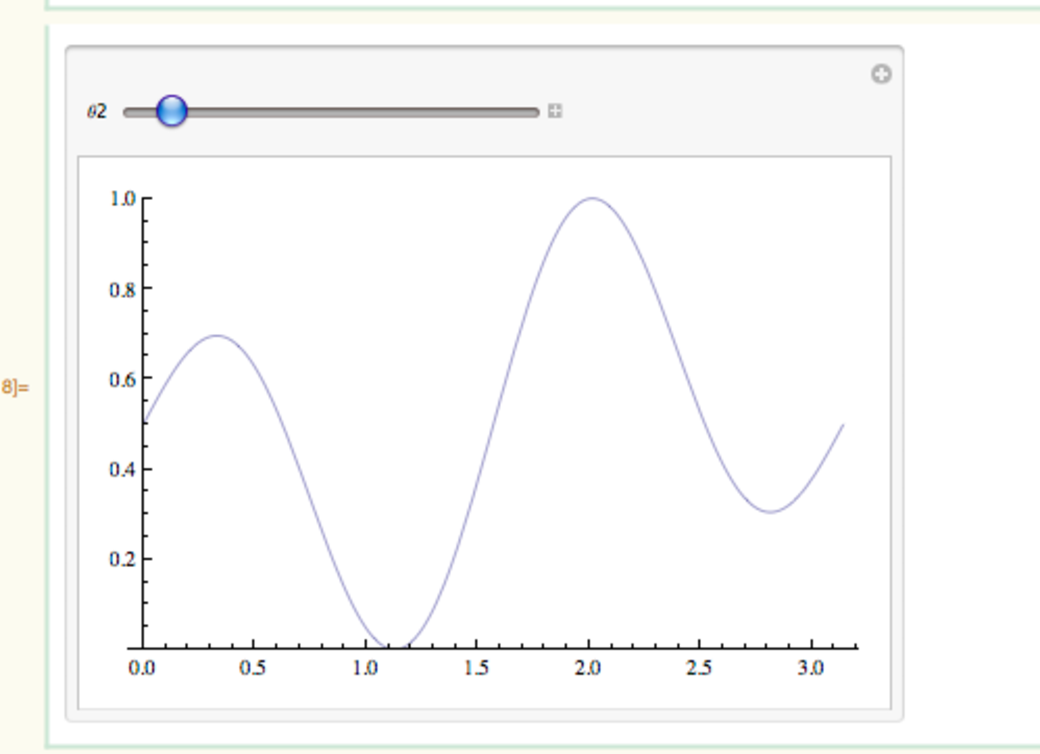
\includegraphics{numericalMethod}}
    \caption[Numerical method]{\label{fig:numericalLightControlMethod}
    Just plot the magnitude of the vertically polarized component as a function of $\theta_1$. I used the slider to control $\theta_2$. Obviously, I'll illustrate this better at some point.}
\end{figure}

We found that when we mount one of the waveplates at angle XXXX, we can adjust the vertical component of the polarization of the outgoing light to anywhere between 0 and one as we adjust it from angle XXXX to YYYY. We did this numerically. 

By physical and numerical experimentation, we found that you can achieve these angles by subsequently adjusting each of the two waveplates in turn. Keeping 100\% of the light vertically polarized is easy and can be achieved for any fixed value of $\theta_2$ since $\theta_1$ can simply be adjusted so that the fast axis of the first waveplate aligns with the slow axis of the second. In this way, the total phase shift experienced by all the components is equal.

Thus, to correctly place the second waveplate at the angle  $\theta_2$, we adjust both angles until the outgoing light is entirely horizontally polarized (as measured by the output of the polarizing beam cube). I found that mounting the waveplates at the approximate angles I calculated followed by alternately adjusting each waveplate to minimize the amount of light transmitted achieved the desired result. 

There is some intuition to be had here. One thing I noticed was that, when the waveplates are adjusted so that the outgoing light is horizontally polarized, the magnitude of the components of light in each polarization between the waveplates is equal. This suggests some symmetry. 

%Consider that, in this part of the setup, we have a time-reversal symmetry. What I mean is, if we send the outgoing light in backwards, we get the incoming light going backwards. Now, I am going to, at some future point write about the following: 

If you have two components of polarization--a horizontal and a vertical with some phase $\phi$ between them, the time reversed wave will have a phase $-\phi$ between its horizontal and vertical components. 

Now, consider the light travelling between the two waveplates (after going through waveplate \#1 but before going through waveplate \#2). 

We first select a rather unusual basis in which to express the Jones vector of this light. We will use the respective polarization vectors of the incoming light and the outgoing light as my basis vectors. These vectors may be non-orthogonal, but they still span the space of all possible polarizations.  

Now, after passing through our first waveplate, the components of polarization as expressed in this basis will have some relative phase offset. 

Now, consider what this would look like time-reversed. If, for example, the phase of the component along the first direction of polarization had a phase $\phi$, the time reversal means that the other component of polarization will be ahead by a phase $\phi$. Now, this is the crux of the argument: 

Consider light with the second desired polarization being sent backwards into the second polarizer. By symmetry, we can orient the second polarizer such that the components of the light, when described in the basis comprised of our unit vectors that point along the directions of the respective fast axes of the two polarizing waveplates 


%maybe do it differentially? You know? 

%let it be imperfect. Use other time for cleverness. Take advantage of having idea net out. 
%should I find a commutator? 
%IDK if I did this right with my \xi
%don't forget to cite peatrossware
%http://www.thorlabs.com/NewGroupPage9.cfm?ObjectGroup_ID=713 is where I got the spreadsheet. 
